% Options for packages loaded elsewhere
% Options for packages loaded elsewhere
\PassOptionsToPackage{unicode}{hyperref}
\PassOptionsToPackage{hyphens}{url}
\PassOptionsToPackage{dvipsnames,svgnames,x11names}{xcolor}
%
\documentclass[
  letterpaper,
  DIV=11,
  numbers=noendperiod]{scrartcl}
\usepackage{xcolor}
\usepackage{amsmath,amssymb}
\setcounter{secnumdepth}{5}
\usepackage{iftex}
\ifPDFTeX
  \usepackage[T1]{fontenc}
  \usepackage[utf8]{inputenc}
  \usepackage{textcomp} % provide euro and other symbols
\else % if luatex or xetex
  \usepackage{unicode-math} % this also loads fontspec
  \defaultfontfeatures{Scale=MatchLowercase}
  \defaultfontfeatures[\rmfamily]{Ligatures=TeX,Scale=1}
\fi
\usepackage{lmodern}
\ifPDFTeX\else
  % xetex/luatex font selection
\fi
% Use upquote if available, for straight quotes in verbatim environments
\IfFileExists{upquote.sty}{\usepackage{upquote}}{}
\IfFileExists{microtype.sty}{% use microtype if available
  \usepackage[]{microtype}
  \UseMicrotypeSet[protrusion]{basicmath} % disable protrusion for tt fonts
}{}
\makeatletter
\@ifundefined{KOMAClassName}{% if non-KOMA class
  \IfFileExists{parskip.sty}{%
    \usepackage{parskip}
  }{% else
    \setlength{\parindent}{0pt}
    \setlength{\parskip}{6pt plus 2pt minus 1pt}}
}{% if KOMA class
  \KOMAoptions{parskip=half}}
\makeatother
% Make \paragraph and \subparagraph free-standing
\makeatletter
\ifx\paragraph\undefined\else
  \let\oldparagraph\paragraph
  \renewcommand{\paragraph}{
    \@ifstar
      \xxxParagraphStar
      \xxxParagraphNoStar
  }
  \newcommand{\xxxParagraphStar}[1]{\oldparagraph*{#1}\mbox{}}
  \newcommand{\xxxParagraphNoStar}[1]{\oldparagraph{#1}\mbox{}}
\fi
\ifx\subparagraph\undefined\else
  \let\oldsubparagraph\subparagraph
  \renewcommand{\subparagraph}{
    \@ifstar
      \xxxSubParagraphStar
      \xxxSubParagraphNoStar
  }
  \newcommand{\xxxSubParagraphStar}[1]{\oldsubparagraph*{#1}\mbox{}}
  \newcommand{\xxxSubParagraphNoStar}[1]{\oldsubparagraph{#1}\mbox{}}
\fi
\makeatother

\usepackage{color}
\usepackage{fancyvrb}
\newcommand{\VerbBar}{|}
\newcommand{\VERB}{\Verb[commandchars=\\\{\}]}
\DefineVerbatimEnvironment{Highlighting}{Verbatim}{commandchars=\\\{\}}
% Add ',fontsize=\small' for more characters per line
\usepackage{framed}
\definecolor{shadecolor}{RGB}{241,243,245}
\newenvironment{Shaded}{\begin{snugshade}}{\end{snugshade}}
\newcommand{\AlertTok}[1]{\textcolor[rgb]{0.68,0.00,0.00}{#1}}
\newcommand{\AnnotationTok}[1]{\textcolor[rgb]{0.37,0.37,0.37}{#1}}
\newcommand{\AttributeTok}[1]{\textcolor[rgb]{0.40,0.45,0.13}{#1}}
\newcommand{\BaseNTok}[1]{\textcolor[rgb]{0.68,0.00,0.00}{#1}}
\newcommand{\BuiltInTok}[1]{\textcolor[rgb]{0.00,0.23,0.31}{#1}}
\newcommand{\CharTok}[1]{\textcolor[rgb]{0.13,0.47,0.30}{#1}}
\newcommand{\CommentTok}[1]{\textcolor[rgb]{0.37,0.37,0.37}{#1}}
\newcommand{\CommentVarTok}[1]{\textcolor[rgb]{0.37,0.37,0.37}{\textit{#1}}}
\newcommand{\ConstantTok}[1]{\textcolor[rgb]{0.56,0.35,0.01}{#1}}
\newcommand{\ControlFlowTok}[1]{\textcolor[rgb]{0.00,0.23,0.31}{\textbf{#1}}}
\newcommand{\DataTypeTok}[1]{\textcolor[rgb]{0.68,0.00,0.00}{#1}}
\newcommand{\DecValTok}[1]{\textcolor[rgb]{0.68,0.00,0.00}{#1}}
\newcommand{\DocumentationTok}[1]{\textcolor[rgb]{0.37,0.37,0.37}{\textit{#1}}}
\newcommand{\ErrorTok}[1]{\textcolor[rgb]{0.68,0.00,0.00}{#1}}
\newcommand{\ExtensionTok}[1]{\textcolor[rgb]{0.00,0.23,0.31}{#1}}
\newcommand{\FloatTok}[1]{\textcolor[rgb]{0.68,0.00,0.00}{#1}}
\newcommand{\FunctionTok}[1]{\textcolor[rgb]{0.28,0.35,0.67}{#1}}
\newcommand{\ImportTok}[1]{\textcolor[rgb]{0.00,0.46,0.62}{#1}}
\newcommand{\InformationTok}[1]{\textcolor[rgb]{0.37,0.37,0.37}{#1}}
\newcommand{\KeywordTok}[1]{\textcolor[rgb]{0.00,0.23,0.31}{\textbf{#1}}}
\newcommand{\NormalTok}[1]{\textcolor[rgb]{0.00,0.23,0.31}{#1}}
\newcommand{\OperatorTok}[1]{\textcolor[rgb]{0.37,0.37,0.37}{#1}}
\newcommand{\OtherTok}[1]{\textcolor[rgb]{0.00,0.23,0.31}{#1}}
\newcommand{\PreprocessorTok}[1]{\textcolor[rgb]{0.68,0.00,0.00}{#1}}
\newcommand{\RegionMarkerTok}[1]{\textcolor[rgb]{0.00,0.23,0.31}{#1}}
\newcommand{\SpecialCharTok}[1]{\textcolor[rgb]{0.37,0.37,0.37}{#1}}
\newcommand{\SpecialStringTok}[1]{\textcolor[rgb]{0.13,0.47,0.30}{#1}}
\newcommand{\StringTok}[1]{\textcolor[rgb]{0.13,0.47,0.30}{#1}}
\newcommand{\VariableTok}[1]{\textcolor[rgb]{0.07,0.07,0.07}{#1}}
\newcommand{\VerbatimStringTok}[1]{\textcolor[rgb]{0.13,0.47,0.30}{#1}}
\newcommand{\WarningTok}[1]{\textcolor[rgb]{0.37,0.37,0.37}{\textit{#1}}}

\usepackage{longtable,booktabs,array}
\usepackage{calc} % for calculating minipage widths
% Correct order of tables after \paragraph or \subparagraph
\usepackage{etoolbox}
\makeatletter
\patchcmd\longtable{\par}{\if@noskipsec\mbox{}\fi\par}{}{}
\makeatother
% Allow footnotes in longtable head/foot
\IfFileExists{footnotehyper.sty}{\usepackage{footnotehyper}}{\usepackage{footnote}}
\makesavenoteenv{longtable}
\usepackage{graphicx}
\makeatletter
\newsavebox\pandoc@box
\newcommand*\pandocbounded[1]{% scales image to fit in text height/width
  \sbox\pandoc@box{#1}%
  \Gscale@div\@tempa{\textheight}{\dimexpr\ht\pandoc@box+\dp\pandoc@box\relax}%
  \Gscale@div\@tempb{\linewidth}{\wd\pandoc@box}%
  \ifdim\@tempb\p@<\@tempa\p@\let\@tempa\@tempb\fi% select the smaller of both
  \ifdim\@tempa\p@<\p@\scalebox{\@tempa}{\usebox\pandoc@box}%
  \else\usebox{\pandoc@box}%
  \fi%
}
% Set default figure placement to htbp
\def\fps@figure{htbp}
\makeatother
\usepackage{svg}





\setlength{\emergencystretch}{3em} % prevent overfull lines

\providecommand{\tightlist}{%
  \setlength{\itemsep}{0pt}\setlength{\parskip}{0pt}}



 


\KOMAoption{captions}{tableheading}
\makeatletter
\@ifpackageloaded{tcolorbox}{}{\usepackage[skins,breakable]{tcolorbox}}
\@ifpackageloaded{fontawesome5}{}{\usepackage{fontawesome5}}
\definecolor{quarto-callout-color}{HTML}{909090}
\definecolor{quarto-callout-note-color}{HTML}{0758E5}
\definecolor{quarto-callout-important-color}{HTML}{CC1914}
\definecolor{quarto-callout-warning-color}{HTML}{EB9113}
\definecolor{quarto-callout-tip-color}{HTML}{00A047}
\definecolor{quarto-callout-caution-color}{HTML}{FC5300}
\definecolor{quarto-callout-color-frame}{HTML}{acacac}
\definecolor{quarto-callout-note-color-frame}{HTML}{4582ec}
\definecolor{quarto-callout-important-color-frame}{HTML}{d9534f}
\definecolor{quarto-callout-warning-color-frame}{HTML}{f0ad4e}
\definecolor{quarto-callout-tip-color-frame}{HTML}{02b875}
\definecolor{quarto-callout-caution-color-frame}{HTML}{fd7e14}
\makeatother
\makeatletter
\@ifpackageloaded{caption}{}{\usepackage{caption}}
\AtBeginDocument{%
\ifdefined\contentsname
  \renewcommand*\contentsname{Table of contents}
\else
  \newcommand\contentsname{Table of contents}
\fi
\ifdefined\listfigurename
  \renewcommand*\listfigurename{List of Figures}
\else
  \newcommand\listfigurename{List of Figures}
\fi
\ifdefined\listtablename
  \renewcommand*\listtablename{List of Tables}
\else
  \newcommand\listtablename{List of Tables}
\fi
\ifdefined\figurename
  \renewcommand*\figurename{Figure}
\else
  \newcommand\figurename{Figure}
\fi
\ifdefined\tablename
  \renewcommand*\tablename{Table}
\else
  \newcommand\tablename{Table}
\fi
}
\@ifpackageloaded{float}{}{\usepackage{float}}
\floatstyle{ruled}
\@ifundefined{c@chapter}{\newfloat{codelisting}{h}{lop}}{\newfloat{codelisting}{h}{lop}[chapter]}
\floatname{codelisting}{Listing}
\newcommand*\listoflistings{\listof{codelisting}{List of Listings}}
\makeatother
\makeatletter
\makeatother
\makeatletter
\@ifpackageloaded{caption}{}{\usepackage{caption}}
\@ifpackageloaded{subcaption}{}{\usepackage{subcaption}}
\makeatother
\makeatletter
\@ifpackageloaded{tikz}{}{\usepackage{tikz}}
\makeatother
        \newcommand*\circled[1]{\tikz[baseline=(char.base)]{
          \node[shape=circle,draw,inner sep=1pt] (char) {{\scriptsize#1}};}}  
                  
\usepackage{bookmark}
\IfFileExists{xurl.sty}{\usepackage{xurl}}{} % add URL line breaks if available
\urlstyle{same}
\hypersetup{
  pdftitle={Ultra (Overpass Ultra) Tutorial},
  pdfauthor={Felipe Valdez},
  colorlinks=true,
  linkcolor={blue},
  filecolor={Maroon},
  citecolor={Blue},
  urlcolor={Blue},
  pdfcreator={LaTeX via pandoc}}


\title{Ultra (Overpass Ultra) Tutorial}
\author{Felipe Valdez}
\date{}
\begin{document}
\maketitle

\renewcommand*\contentsname{Contents}
{
\hypersetup{linkcolor=}
\setcounter{tocdepth}{3}
\tableofcontents
}

\begin{figure}[H]

{\centering \pandocbounded{\includesvg[keepaspectratio]{ultra_tutorial_files/mediabag/zenodo.17343164.svg}}

}

\caption{DOI}

\end{figure}%

Cite this tutorial: Valdez, Felipe. (2025, March 7). Ultra (overpass
ultra) Tutorial v1.0. Zenodo. https://doi.org/10.5281/zenodo.17343164

\section{What is Ultra?}\label{what-is-ultra}

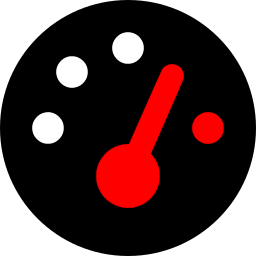
\includegraphics[width=1.04167in,height=\textheight,keepaspectratio]{./images/ultra-logo.png}

\href{https://overpass-ultra.us/docs/}{Ultra} (née Overpass Ultra) is a
web-application made to simplify making maps with
\href{https://maplibre.org/maplibre-gl-js/docs/}{MapLibre GL JS} with
data from various file/query types such as Overpass, GeoJSON, GPX, and
more.

\section{What is Overpass?}\label{what-is-overpass}

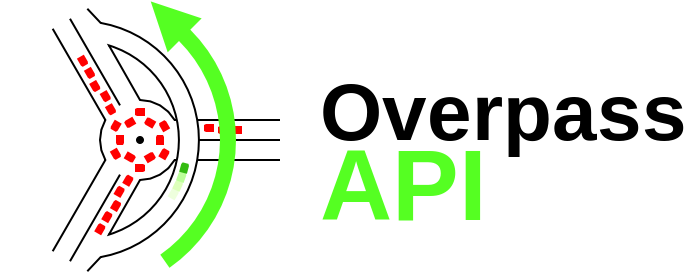
\includegraphics[width=2.60417in,height=\textheight,keepaspectratio]{./images/overpass_logo.png}

The \href{https://wiki.openstreetmap.org/wiki/Overpass_API}{Overpass
API} is a read-only service that lets users retrieve specific
\href{https://www.openstreetmap.org/}{OpenStreetMap} (OSM) data based on
custom queries.

Unlike OSM's main API, which focuses on editing, Overpass is optimized
for data retrieval, handling anything from a few elements to millions in
minutes.

Users can filter data by location, object type, tags, and more. Overpass
Ultra, a web-based tool, helps with query creation.

Refer to the \href{https://dev.overpass-api.de/overpass-doc/en/}{user
manual} and
\href{https://wiki.openstreetmap.org/wiki/Overpass_API/Overpass_QL}{Overpass
QL guide} for details.

\textbf{Resulting map from this tutorial}

\href{https://overpass-ultra.us/\#map&m=13.07/39.9596/-75.1743&q=LQhQBcEtwGwUwFwAIBKcDGAnOBDKB7AOxxiR2xwGclJCkAFAC0hhwBM4YAHZnUDylkhcChZAFkcXJPgBmZGKWxZcokmQrVaScIzhJ00AJ4z5TFu049IfLvi4BXLgHlCACXwA3OJmThMDnCgdo5cACpwALZcrOCISABEAN5J4DgA5pQAdMSRcAC++UjASClpmVnwkJQO2IUJoPailAigSAZwhHG+SADaxQDsAKxZAIwDACyTADRIAMwAnFkLQwAcqwAMSAC6bUgAXvj4kcijc1mrc6DoRP74MC17JeBGXPEAcjiekOl4kEQAYVumHue3adko0H+Yh09mAmB+jHATx0r3iAHE4Pd8Og8HAgV0QTAwTIRNDHu1KUgIVCiM4yUQKVTKZ0cAAjeBuREAQXQ6FqOHQRj8ASCzJ0mEFAGsAKqUHwAGRxfyIIsCKJeb2QbjC4gVBLuxKpTXJrXFSMiMGQAD4SVSADyMUbW+3oTrda3o7CdDS4LR0cysDjcXj2gD0bq6PhdYadtvF6EoLSQ8fFSCdpTtzJpomQskgAA84GwANxZqngezIDZltOU+CycDV2t1pAI9JI5vlpD5UCUF7wM1IVhGHxM9rPNF5lhG7M4WhN7v5xTAG4wfC+bsTgxUMWtkr9AC8h9m-XScHAsyqNWwO1mCS45ClCR2W+KbfSbIAFKMhgtZgATFMswDAAlEgADESDpN6hBvgeSDHqe0EXlecDVLU+jbPeMQ4EYMH4A4hBsC+uytu+mCfl+myzKMABscyzAsozgVBbBPtB2BweRCFIX0KGXsO6E3lh96-JgHCEKR8Eft+oyrKMtF-rRdGsUgbIggA7tx+6yV+GyzAZSAbKBexwAWcTEcmSLgFwLRhmG-ZGPA2T+PODxpFklCMGGXAgpWkRSJQwAwIi4BZAAVpQRCgCAwCgL0bJsvgBYICkSUpYU2xll+eyEJpmC9NemGHo+mBStleUFUVwklbh+EgkRbCVe0+WFcV2CHuJkmVaBZaEeAKHHCWQA}{Open
the resulting map in a new window}

\section{Building an overpass query}\label{building-an-overpass-query}

In this step-by-step tutorial we will learn how to create, style and
share a map in Ultra.

We will be creating an interactive map of all recreation areas in
Philadelphia.

{01} \emph{Open a new map in Ultra}

Go to \url{https://overpass-ultra.us/}.

The first time you open the web you will see a default map like this:

\pandocbounded{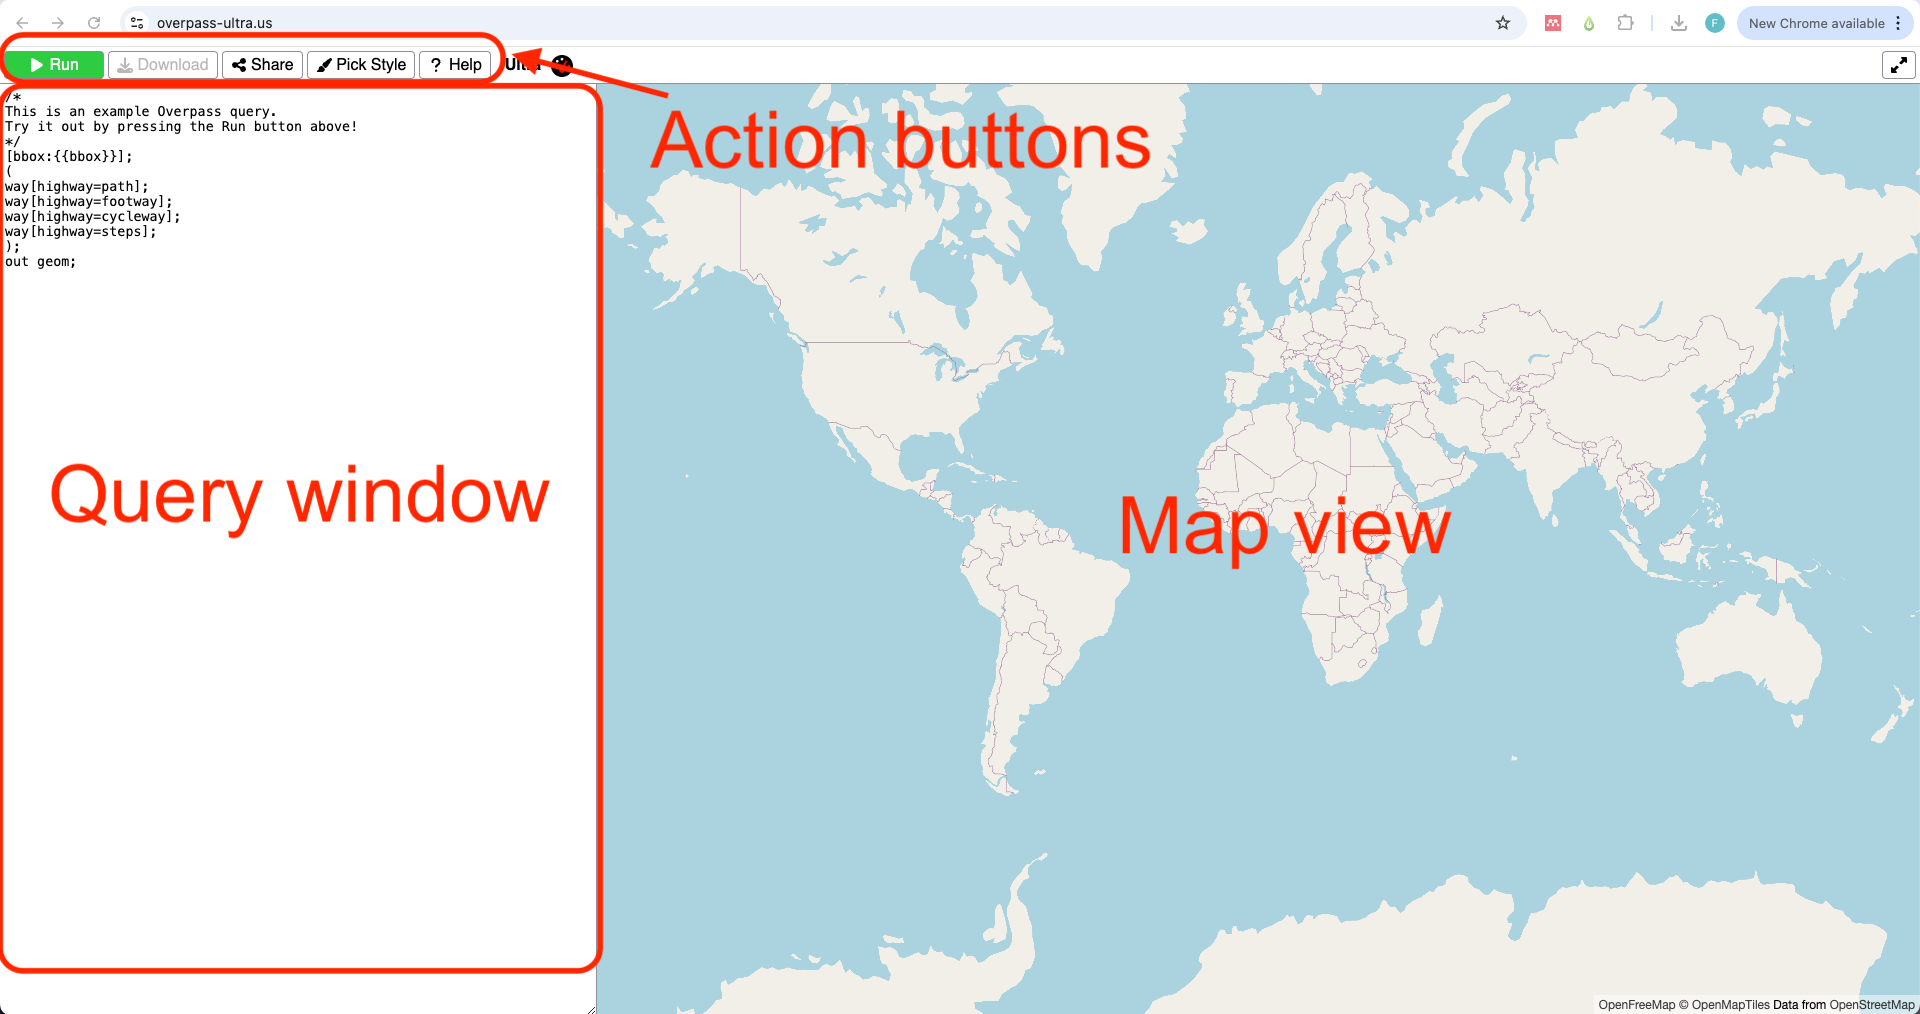
\includegraphics[keepaspectratio]{./images/ultra-screen1.png}}

{02} \emph{Type your query}

A \texttt{query} is a way to filter and retrieve data from
OpenStreetMap. It allows you to search for specific types of map
features.

Queries in Ultra follow the strcuture of the
\href{https://wiki.openstreetmap.org/wiki/Overpass_API}{Overpass API}.

If you are not familiar with OpenStreetMap data, see the info window
below:

\begin{tcolorbox}[enhanced jigsaw, opacitybacktitle=0.6, colback=white, titlerule=0mm, colbacktitle=quarto-callout-caution-color!10!white, coltitle=black, title=\textcolor{quarto-callout-caution-color}{\faFire}\hspace{0.5em}{How data is organized in OSM?}, leftrule=.75mm, breakable, bottomrule=.15mm, opacityback=0, bottomtitle=1mm, toprule=.15mm, toptitle=1mm, colframe=quarto-callout-caution-color-frame, arc=.35mm, rightrule=.15mm, left=2mm]

All data in OSM is represented by an \textbf{element.}

An \textbf{element} can be either a \texttt{node}
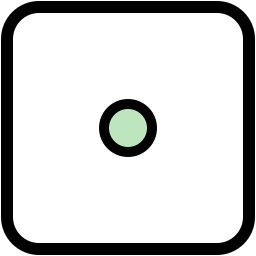
\includegraphics[width=0.03\linewidth,height=\textheight,keepaspectratio]{./images/Osm_element_node.png},
a \texttt{way}
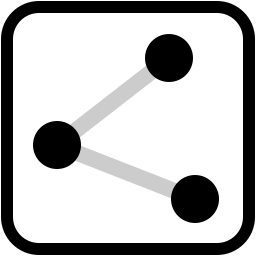
\includegraphics[width=0.03\linewidth,height=\textheight,keepaspectratio]{./images/Osm_element_way.png}
or a \texttt{relation}
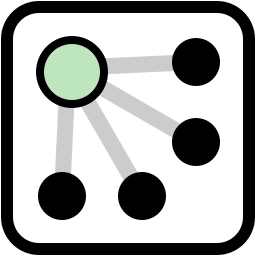
\includegraphics[width=0.03\linewidth,height=\textheight,keepaspectratio]{./images/Osm_element_relation.png}.

Each element is described using \texttt{tags} which are the combination
of a \texttt{key} and a \texttt{value}
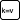
\includegraphics[width=0.3125in,height=0.3125in]{./images/Mf_tag.png}.

For example, a coffee shop is represented by an element type
\texttt{node} with tags \texttt{amenity=cafe}.

Learn more about elements and tags
\href{https://wiki.openstreetmap.org/wiki/Elements}{here.}

\end{tcolorbox}

\textbf{The `anatomy' of a query:} \emph{Hover over the numbers on the
right in the code to reveal what each line on the query does}

The following is the default query you see when you open Ultra for the
first time:

\phantomsection\label{annotated-cell-1}%
\begin{Shaded}
\begin{Highlighting}[numbers=left,,]
\CommentTok{/* }\hspace*{\fill}\NormalTok{\circled{1}}


\CommentTok{*/}\NormalTok{ \# }\OperatorTok{\textless{}}\DecValTok{1}\OperatorTok{\textgreater{}}
\NormalTok{[bbox}\OperatorTok{:}\NormalTok{\{\{bbox\}\}]}\OperatorTok{;}\NormalTok{ \# }\OperatorTok{\textless{}}\DecValTok{2}\OperatorTok{\textgreater{}}
\NormalTok{(                                               }
\NormalTok{way[highway}\OperatorTok{=}\NormalTok{path]}\OperatorTok{;}\NormalTok{ \# }\OperatorTok{\textless{}}\DecValTok{3}\OperatorTok{\textgreater{}}
\NormalTok{way[highway}\OperatorTok{=}\NormalTok{footway]}\OperatorTok{;}
\NormalTok{way[highway}\OperatorTok{=}\NormalTok{cycleway]}\OperatorTok{;}
\NormalTok{way[highway}\OperatorTok{=}\NormalTok{steps]}\OperatorTok{;}
\NormalTok{)}\OperatorTok{;}\NormalTok{ \# }\OperatorTok{\textless{}}\DecValTok{4}\OperatorTok{\textgreater{}}
\NormalTok{out geom}\OperatorTok{;}\NormalTok{ \# }\OperatorTok{\textless{}}\DecValTok{5}\OperatorTok{\textgreater{}}
\end{Highlighting}
\end{Shaded}

\begin{description}
\tightlist
\item[\circled{1}]
This is a comment. Everithing inside \texttt{/*\ \ */} will not be
considered in teh query.
\item[\circled{2}]
This lines defines a \texttt{bbox} which limits the query to what you
are viewing on the map.
\item[\circled{3}]
This line retrieves an element type \texttt{way} that has the key
\texttt{highway} and value \texttt{path}.
\item[\circled{4}]
All single queries within the \texttt{()} are grouped together.
\item[\circled{5}]
The output format for your query. In this case \texttt{geom} returns the
actual shape of the features.
\end{description}

For this example we will use the following query.

As there are different types of recreational areas, we will be using a
group of three queries with different combinations of value for the key
\texttt{leisure}. We will be quering elements tagged:
\texttt{"leisure":"park"}, \texttt{"leisure":"playground"} and
\texttt{"leisure":"garden"}. There are more tags that can describe this
areas. Explore your own case study in \href{openstreetmap.org}{OSM}.

\begin{tcolorbox}[enhanced jigsaw, opacitybacktitle=0.6, colback=white, titlerule=0mm, colbacktitle=quarto-callout-note-color!10!white, coltitle=black, title=\textcolor{quarto-callout-note-color}{\faInfo}\hspace{0.5em}{Note}, leftrule=.75mm, breakable, bottomrule=.15mm, opacityback=0, bottomtitle=1mm, toprule=.15mm, toptitle=1mm, colframe=quarto-callout-note-color-frame, arc=.35mm, rightrule=.15mm, left=2mm]

\textbf{Remember} to zoom in to your ineterest area. Keep your query
area small to retrieve data faster.

\end{tcolorbox}

\phantomsection\label{annotated-cell-2}%
\begin{Shaded}
\begin{Highlighting}[numbers=left,,]
\NormalTok{[bbox}\OperatorTok{:}\NormalTok{\{\{bbox\}\}]}\OperatorTok{;}\NormalTok{ \# }\OperatorTok{\textless{}}\DecValTok{6}\OperatorTok{\textgreater{}}
\NormalTok{( \# }\OperatorTok{\textless{}}\DecValTok{7}\OperatorTok{\textgreater{}}
\NormalTok{nwr[leisure}\OperatorTok{=}\StringTok{"park"}\NormalTok{]}\OperatorTok{;}\NormalTok{ \# }\OperatorTok{\textless{}}\DecValTok{8}\OperatorTok{\textgreater{}}
\NormalTok{nwr[leisure}\OperatorTok{=}\StringTok{"playground"}\NormalTok{]}\OperatorTok{;}\NormalTok{ \# }\OperatorTok{\textless{}}\DecValTok{9}\OperatorTok{\textgreater{}}
\NormalTok{nwr[leisure}\OperatorTok{=}\StringTok{"garden"}\NormalTok{]}\OperatorTok{;}\NormalTok{ \# }\OperatorTok{\textless{}}\DecValTok{10}\OperatorTok{\textgreater{}}
\NormalTok{)}\OperatorTok{;}
\NormalTok{out geom}\OperatorTok{;}\NormalTok{ \# }\OperatorTok{\textless{}}\DecValTok{11}\OperatorTok{\textgreater{}}
\end{Highlighting}
\end{Shaded}

\begin{description}
\tightlist
\item[\circled{6}]
We will keep the \texttt{{[}bbox:\{\{bbox\}\}{]};} line to filter the
query to the map view.
\item[\circled{7}]
Here we start our grouped query. As there are different types of areas,
we will be using three values.
\item[\circled{8}]
One way to tag recreational areas is \texttt{leisure:"park"}. Note that
we use \texttt{nwr} to get any \texttt{node}, \texttt{way} or
\texttt{relation}.
\item[\circled{9}]
Our second query is \texttt{leisure:"playground"}.
\item[\circled{10}]
The third type we are quering is \texttt{leisure:"garden"}.
\item[\circled{11}]
We close our query retrieving the geomtery of the elements.
\end{description}

{03} \emph{Run your query}

Copy and paste this query in Ultra's query window, and then click `Run'
\pandocbounded{
\includegraphics[keepaspectratio]{./images/ultra-run.png}}

\pandocbounded{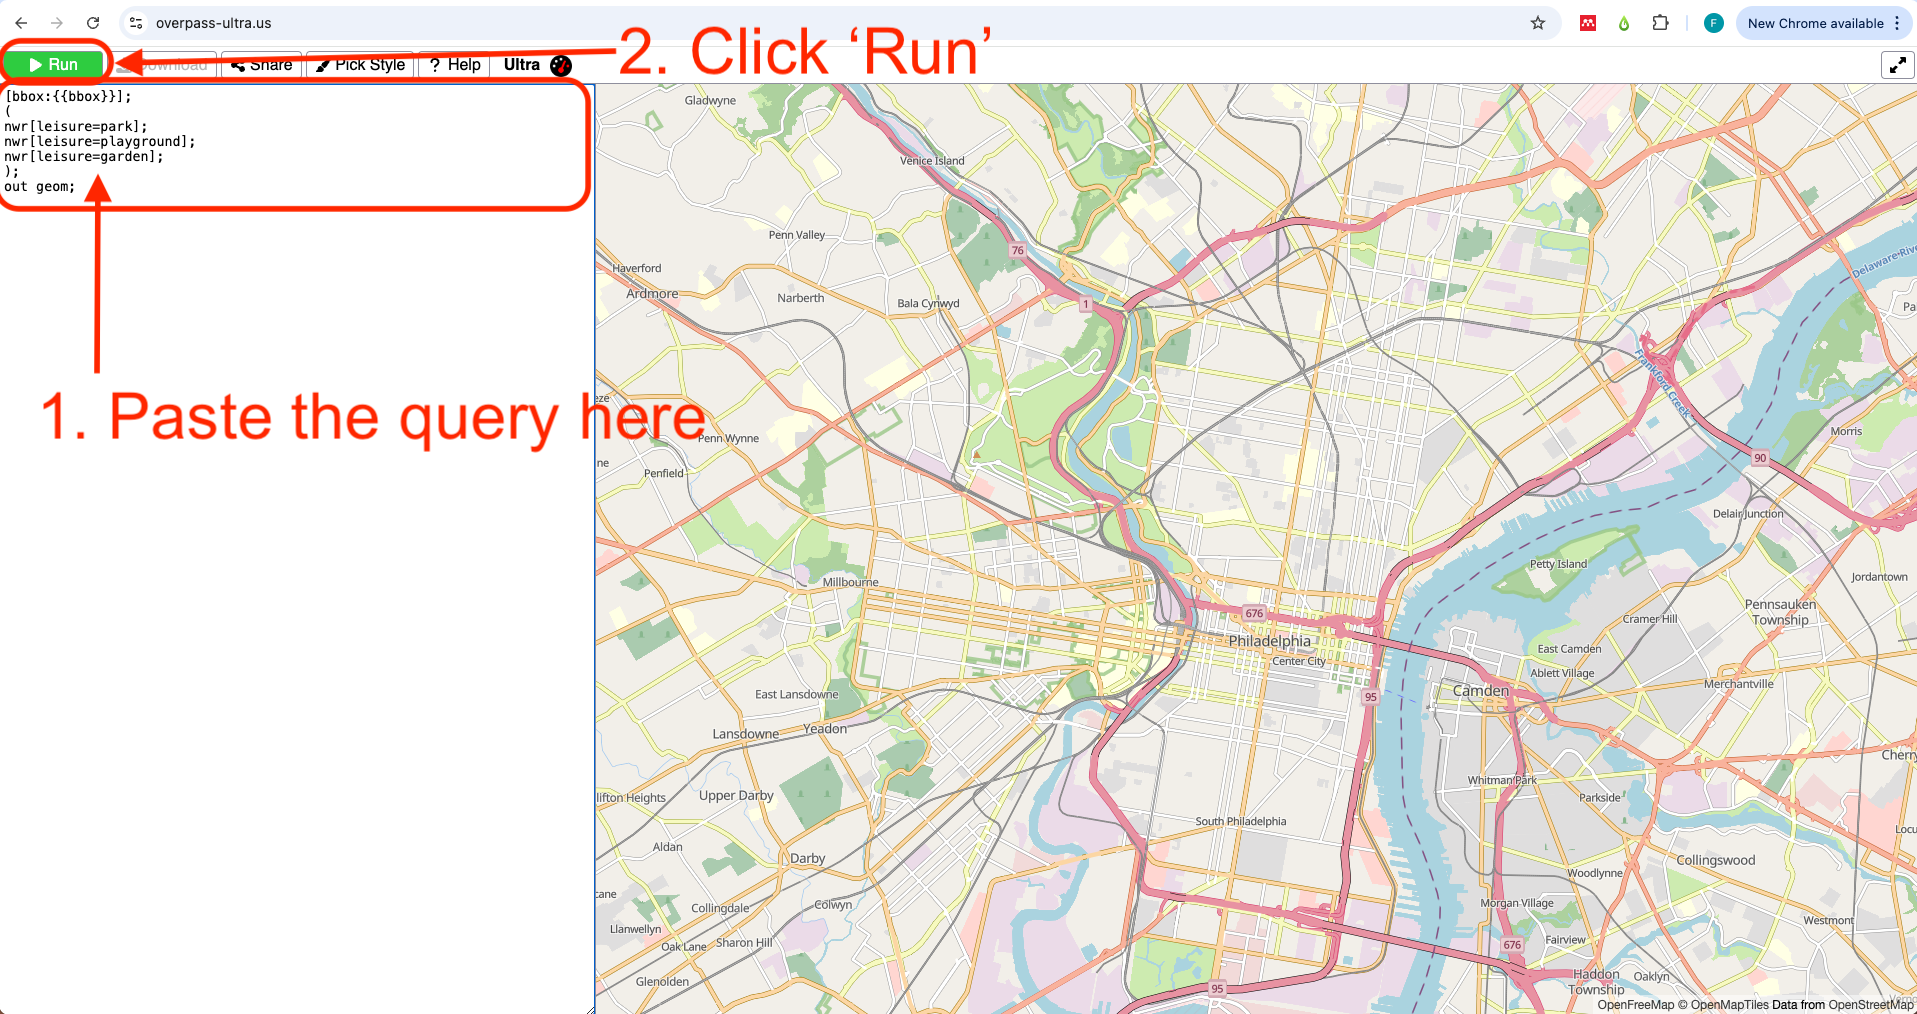
\includegraphics[keepaspectratio]{./images/ultra-screen2.png}}

After some seconds you will see the results display on the map. All
results are shown in yellow. In the next steps we will learn how to
style the results.

Learn more on how to build a query \href{}{here}

\section{Styling in Ultra}\label{styling-in-ultra}

In Ultra, you can style the map elements by adding a \texttt{style:} key
on a YAML front-matter. This YAML front-matter is a way to add metadata
to the query file. All these will be read by Maplibre and Ultra when
rendering your resulting map.

{01} \emph{Add a title and description}

The YAML front-matter has to be framed inside \texttt{-\/-\/-}, just
like in the example below.

\phantomsection\label{annotated-cell-3}%
\begin{Shaded}
\begin{Highlighting}[numbers=left,,]
\NormalTok{{-}{-}{-} \# }\ErrorTok{\textless{}}\NormalTok{1\textgreater{}}
\NormalTok{title: Recreational areas in Philadelphia \# }\ErrorTok{\textless{}}\NormalTok{2\textgreater{}}
\NormalTok{description: Map of all recreational areas in the city of Philadelphia \# }\ErrorTok{\textless{}}\NormalTok{3\textgreater{}}
\NormalTok{{-}{-}{-} \# }\ErrorTok{\textless{}}\NormalTok{4\textgreater{}}
\end{Highlighting}
\end{Shaded}

\begin{description}
\tightlist
\item[\circled{1}]
Opening the YAML front-matter text.
\item[\circled{2}]
Title property to be incldued.
\item[\circled{3}]
Description text to be included.
\item[\circled{4}]
Closing line of the YAML front-matter.
\end{description}

Copy and paste (or type) the YAML front-matter with the title and
description properties into the Ultra query we created in the previous
section.

Paste the YAML front-matter \textbf{before} the query text.

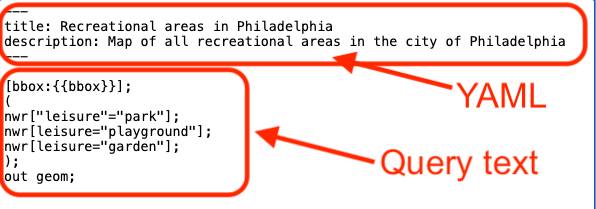
\includegraphics[width=4.375in,height=\textheight,keepaspectratio]{./images/ultra-yaml.png}

{02} \emph{Add a custom style}

Styling is possible in Ultra within the YAML front-matter. A
\texttt{style} is a series of rules on how to visually render a map,
what elements are drawn and which colors, icons, sizes, and more to use.

Ultra uses the \href{https://maplibre.org/maplibre-style-spec/}{Maplibre
Style Spec}. This style is specified by \texttt{properties}.

In this section we describe some of the basic \texttt{properties} needed
to create a custom style.

The first step is to add \texttt{style:} to the YAML front-matter. You
can tyoe it right after the \texttt{description:} property.

We will assign colors to the polygons we obtained from the query. For
that we will add a layer of type fill (polygon) with
\texttt{-\ type:\ fill}. There are other types of layers you can add:
`background', `circle', `heatmap', `fill-extrusion', `line', `symbol'.
Each serves different purposes and works for specific elements, if it is
a point, for example, you might use type:symbol.

Then we specify the property of our layer of type `fill' we want to
modify.

We add \texttt{fill-color:} to change the color of our polygons. Each
layer type has its own properties that can be modified. See
\href{https://maplibre.org/maplibre-style-spec/layers/\#fill}{Layes} on
the Maplibre Style Spec documentation.

{03} \emph{Add conditionals to assign colors based on the feature
properties}

Since we want to color each type of recreational area with a different
color, we are using \texttt{-\ case} (line 9) to introduce conditions.
We type a conditional statement followed by a specific color for each
type of recreational area.

On line 10 of the example code we add \texttt{{[}get,\ leisure{]}} to
select the tag \texttt{leisure} from the proeprties. Then we ask for
those elements that have \texttt{"park"} as the value for that tag. The
\texttt{==} symbol states this.

On line 11, we specify the color we want to assign to the polygons with
tag \texttt{leisure=park}. The colors can be specified using the `rgb'
(red, green, blue) format. You can use tools like
\href{https://www.google.com/search?q=google+color+picker&oq=google+color&gs_lcrp=EgZjaHJvbWUqDQgFEAAYgwEYsQMYgAQyEAgAEAAYkQIYsQMYgAQYigUyBggBEEUYOTINCAIQABiRAhiABBiKBTINCAMQABiRAhiABBiKBTINCAQQABiRAhiABBiKBTINCAUQABiDARixAxiABDIHCAYQABiABDIHCAcQABiABDIHCAgQABiABDIHCAkQABiABNIBCDYyODBqMGo5qAIAsAIB&sourceid=chrome&ie=UTF-8}{Google
Color Picker} to know the `rgb' code of a color.

Lines 12 to 15 on the sample code contain the same conditional + color
for the other two types of recreational areas: playground and garden.

On line 16 we introduce a fallback color. This color will be assigned to
polygons that do not satisfy the conditions in our \texttt{case}. You
always need to assign a fallback color in Maplibre Style Spec.

{04} \emph{Run the query again}

Copy and paste the sample code below on your Ultra map and run the query
again.

\phantomsection\label{annotated-cell-4}%
\begin{Shaded}
\begin{Highlighting}[numbers=left,,]
\OperatorTok{{-}{-}{-}}
\NormalTok{title}\OperatorTok{:}\NormalTok{ Recreational areas }\KeywordTok{in}\NormalTok{ Philadelphia}
\NormalTok{description}\OperatorTok{:}\NormalTok{ Map }\KeywordTok{of}\NormalTok{ all recreational areas }\KeywordTok{in}\NormalTok{ the city }\KeywordTok{of}\NormalTok{ Philadelphia}
\NormalTok{style}\OperatorTok{:}\NormalTok{ \# }\OperatorTok{\textless{}}\DecValTok{1}\OperatorTok{\textgreater{}}
\NormalTok{  layers}\OperatorTok{:}\NormalTok{ \# }\OperatorTok{\textless{}}\DecValTok{2}\OperatorTok{\textgreater{}}
    \OperatorTok{{-}}\NormalTok{ type}\OperatorTok{:}\NormalTok{ fill \# }\OperatorTok{\textless{}}\DecValTok{3}\OperatorTok{\textgreater{}}
\NormalTok{      paint}\OperatorTok{:}\NormalTok{ \# }\OperatorTok{\textless{}}\DecValTok{4}\OperatorTok{\textgreater{}}
\NormalTok{        fill}\OperatorTok{{-}}\NormalTok{color}\OperatorTok{:}\NormalTok{ \# }\OperatorTok{\textless{}}\DecValTok{5}\OperatorTok{\textgreater{}}
          \OperatorTok{{-}} \ControlFlowTok{case}\NormalTok{ \# }\OperatorTok{\textless{}}\DecValTok{6}\OperatorTok{\textgreater{}}
          \OperatorTok{{-}}\NormalTok{ [ }\OperatorTok{==,}\NormalTok{ [ }\KeywordTok{get}\OperatorTok{,}\NormalTok{ leisure ]}\OperatorTok{,} \StringTok{"park"}\NormalTok{ ] \# }\OperatorTok{\textless{}}\DecValTok{7}\OperatorTok{\textgreater{}}
          \OperatorTok{{-}} \FunctionTok{rgb}\NormalTok{(}\DecValTok{159}\OperatorTok{,} \DecValTok{247}\OperatorTok{,} \DecValTok{7}\NormalTok{) \# green \# }\OperatorTok{\textless{}}\DecValTok{8}\OperatorTok{\textgreater{}}
          \OperatorTok{{-}}\NormalTok{ [ }\OperatorTok{==,}\NormalTok{ [ }\KeywordTok{get}\OperatorTok{,}\NormalTok{ leisure ]}\OperatorTok{,} \StringTok{"playground"}\NormalTok{ ] \# }\OperatorTok{\textless{}}\DecValTok{9}\OperatorTok{\textgreater{}}
          \OperatorTok{{-}} \FunctionTok{rgb}\NormalTok{(}\DecValTok{80}\OperatorTok{,} \DecValTok{163}\OperatorTok{,} \DecValTok{91}\NormalTok{) \# dark gren \# }\OperatorTok{\textless{}}\DecValTok{9}\OperatorTok{\textgreater{}}
          \OperatorTok{{-}}\NormalTok{ [ }\OperatorTok{==,}\NormalTok{ [ }\KeywordTok{get}\OperatorTok{,}\NormalTok{ leisure ]}\OperatorTok{,} \StringTok{"garden"}\NormalTok{ ] \# }\OperatorTok{\textless{}}\DecValTok{9}\OperatorTok{\textgreater{}}
          \OperatorTok{{-}} \FunctionTok{rgb}\NormalTok{(}\DecValTok{181}\OperatorTok{,} \DecValTok{159}\OperatorTok{,} \DecValTok{16}\NormalTok{) \# brown \# }\OperatorTok{\textless{}}\DecValTok{9}\OperatorTok{\textgreater{}}
          \OperatorTok{{-}} \FunctionTok{rgb}\NormalTok{(}\DecValTok{0}\OperatorTok{,} \DecValTok{0}\OperatorTok{,} \DecValTok{0}\NormalTok{) \# }\OperatorTok{\textless{}}\DecValTok{10}\OperatorTok{\textgreater{}}
\OperatorTok{{-}{-}{-}}
\NormalTok{[bbox}\OperatorTok{:}\NormalTok{\{\{bbox\}\}]}\OperatorTok{;}
\NormalTok{(}
\NormalTok{  nwr[leisure}\OperatorTok{=}\NormalTok{park]}\OperatorTok{;}
\NormalTok{  nwr[leisure}\OperatorTok{=}\NormalTok{playground]}\OperatorTok{;}
\NormalTok{  nwr[leisure}\OperatorTok{=}\NormalTok{garden]}\OperatorTok{;}
\NormalTok{)}\OperatorTok{;}
\NormalTok{out geom}\OperatorTok{;}
\end{Highlighting}
\end{Shaded}

\begin{description}
\tightlist
\item[\circled{1}]
We start the style section with this line.
\item[\circled{2}]
The most important property is \texttt{layers} which adds something to
the map.
\item[\circled{3}]
We define our layer type as \texttt{fill} as we want the polygons to be
painted in the map.
\item[\circled{4}]
There are two main types of properties \texttt{paint:} and
\texttt{layout}.
\item[\circled{5}]
We define the \texttt{fill-color} to be the property we want to modify.
\item[\circled{6}]
The \texttt{case} expression will assign a value to an output of a
condition (lines 10 to 15).
\item[\circled{7}]
We search for features that have \texttt{park} as the value of
\texttt{leisure}.
\item[\circled{8}]
This color is assigned to those features that satisfy the condition
established in the previous line.
\item[\circled{9}]
We do the same evaluation and assignment for thos features with
\texttt{playground} (line 13) and \texttt{garden} (line 15).
\item[\circled{10}]
This is the fallback color. This will be assigned if there are features
that do not satisfy any of the previous conditions.
\end{description}

\pandocbounded{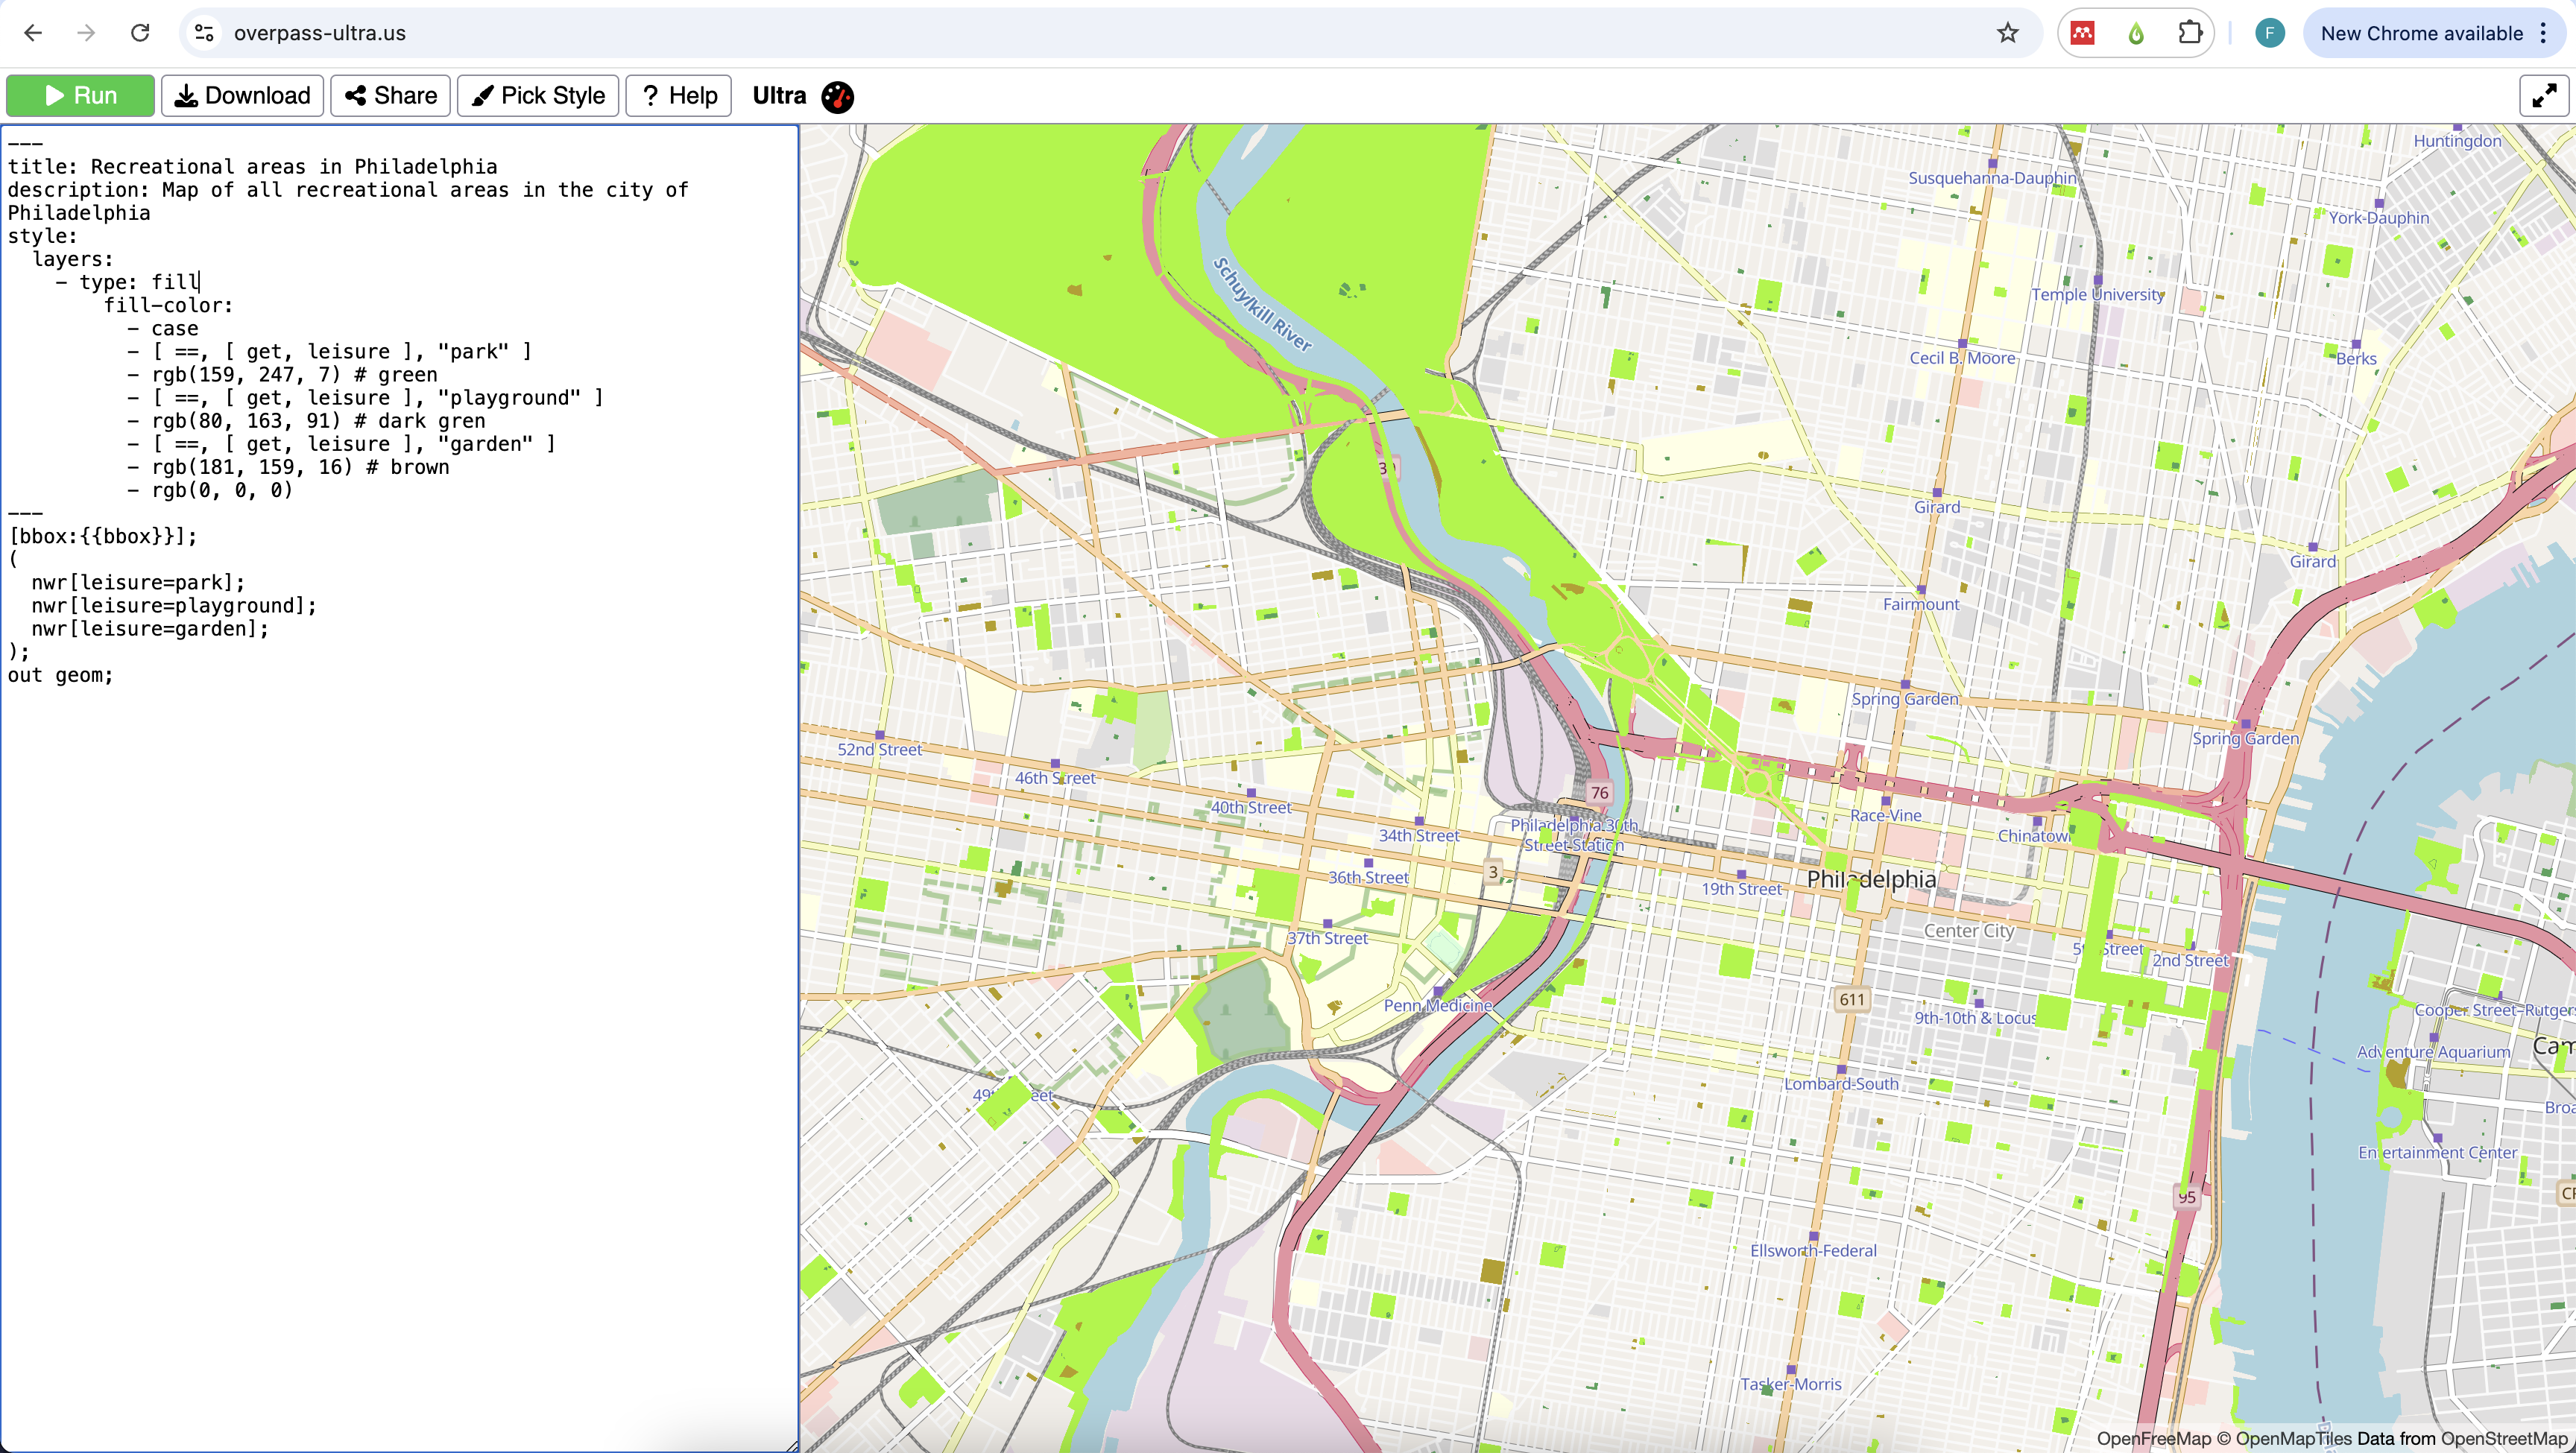
\includegraphics[keepaspectratio]{./images/ultra-screen3.png}}

{05} \emph{Change the background style}

Ultra comes with a variety of background styles you can choose. To
change the style click on the \href{./images/ultra-pick.png}{Pick Style}
button on the top menu bar and select any style from the list.

In this example we chose `Protomaps Light' because it uses shadows of
grey for most of the elements, highlighting the vibrant greens we chose
for the parks.

\pandocbounded{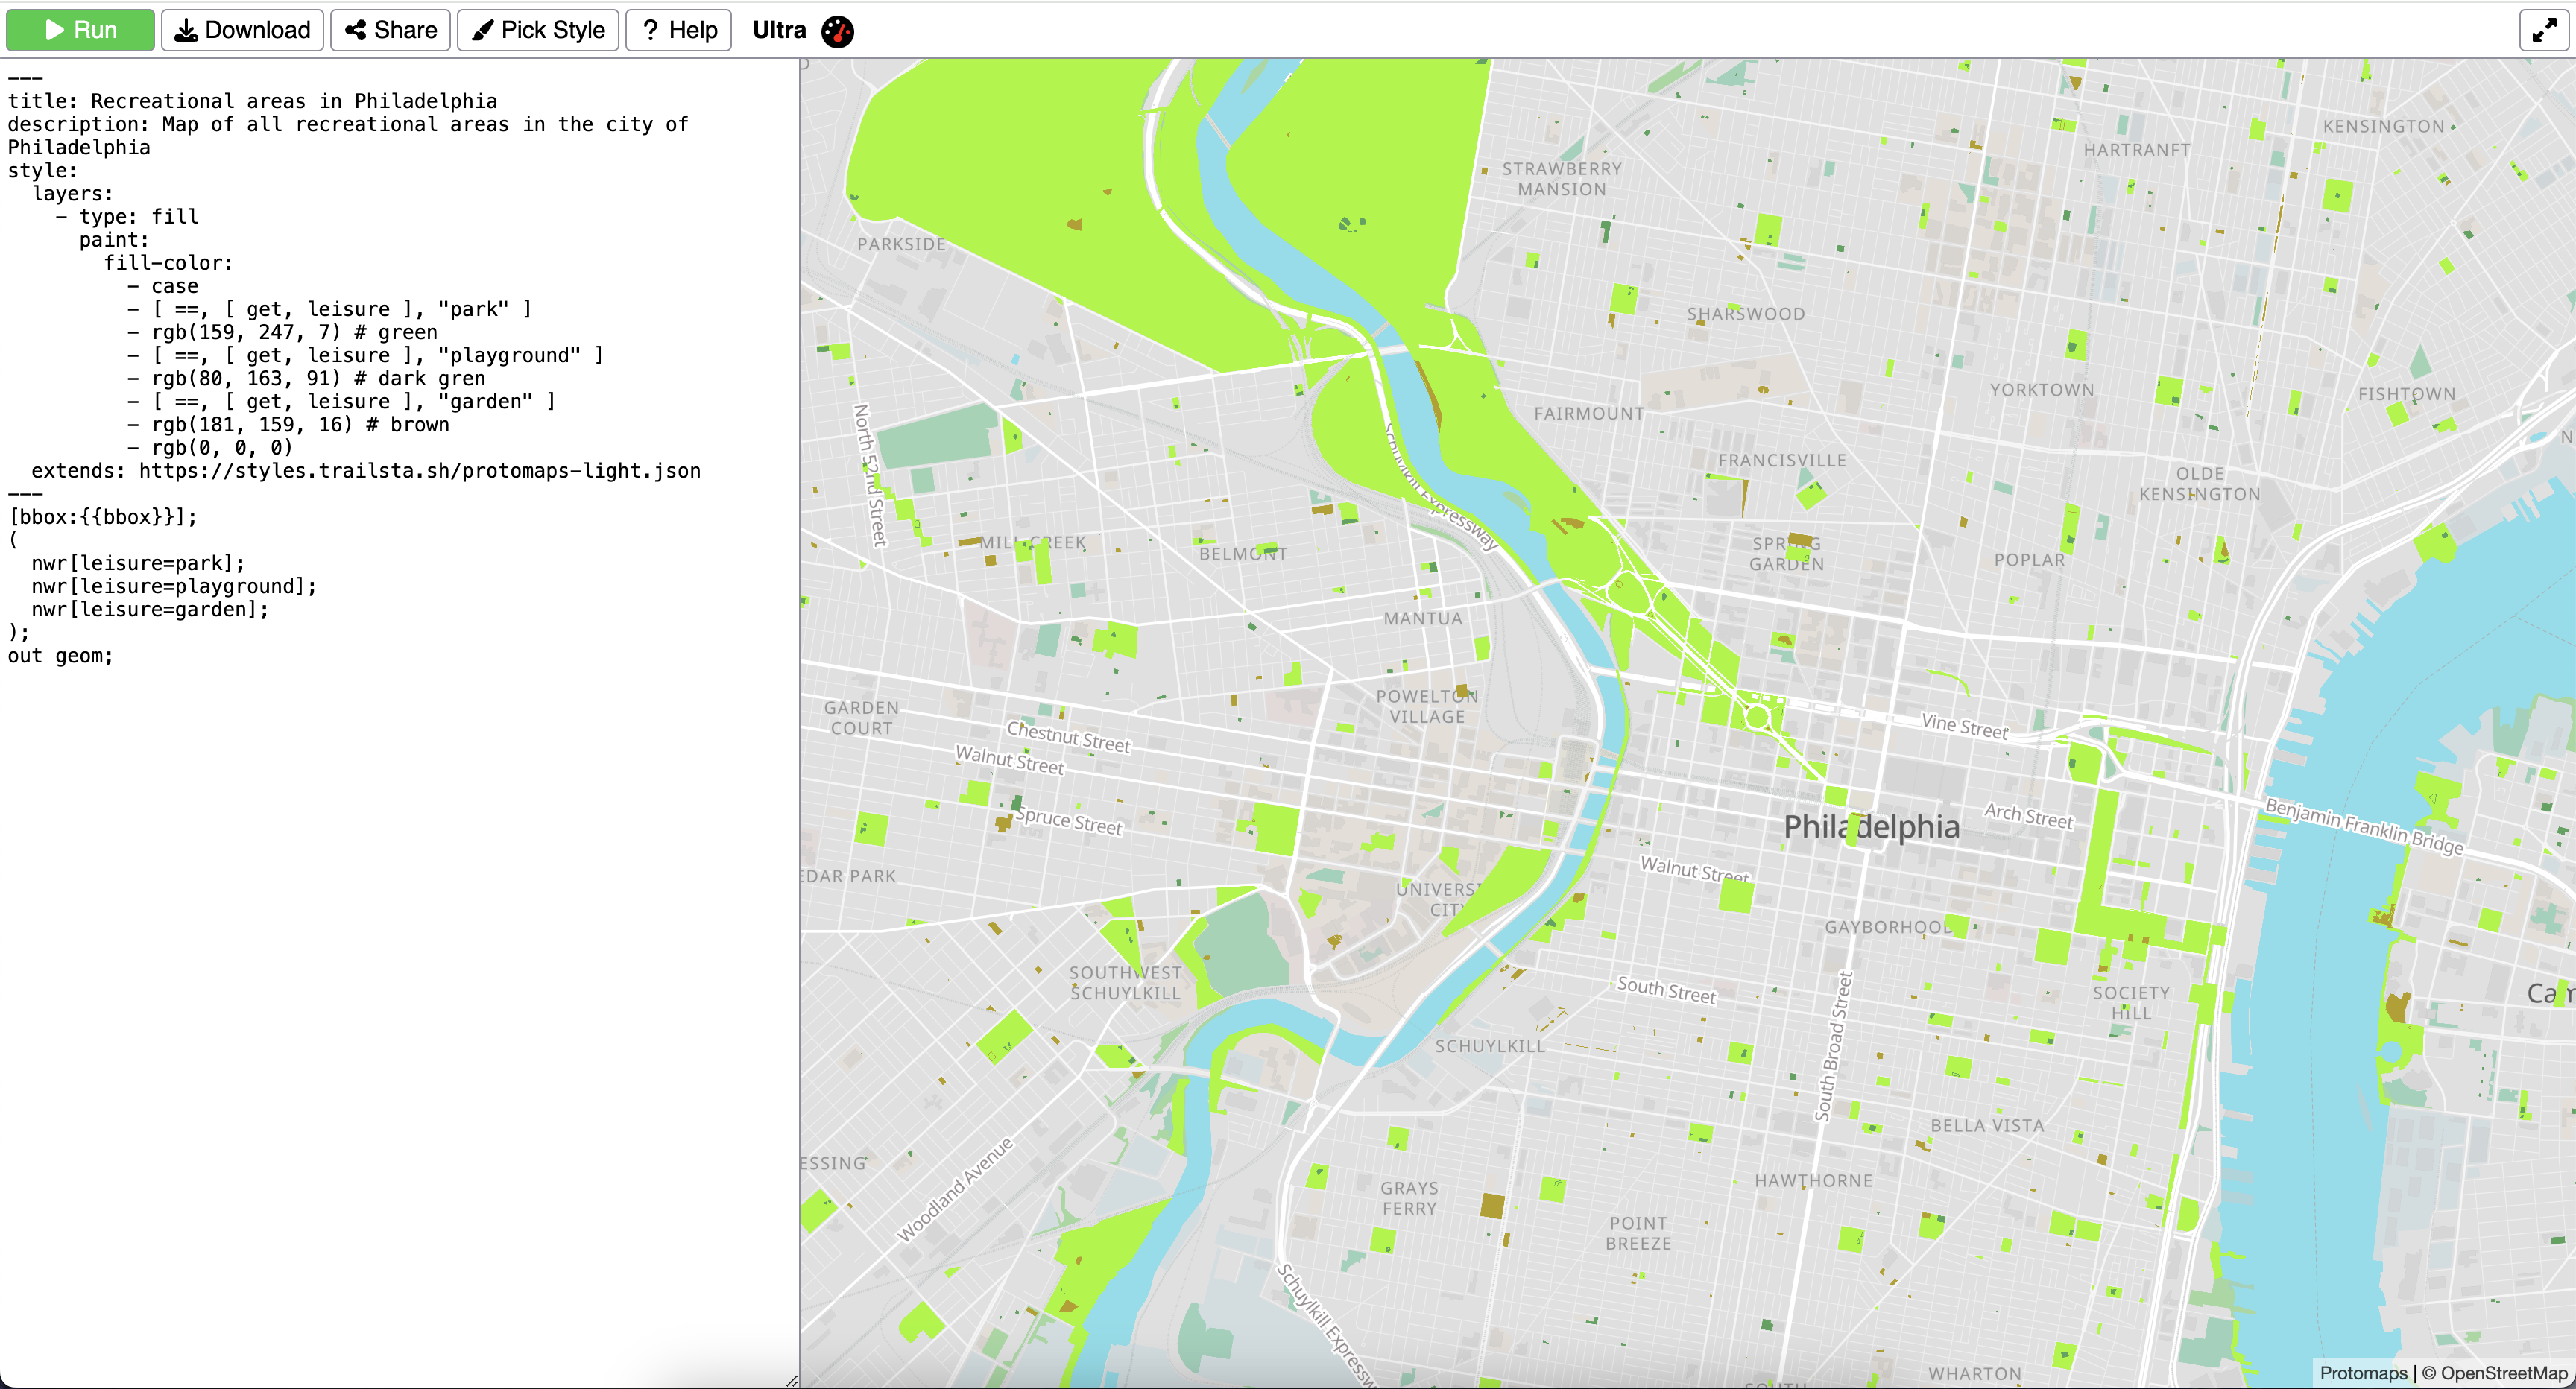
\includegraphics[keepaspectratio]{./images/ultra-screen4.png}}

Notice that an extra line is added to the YAML front-matter with the URL
of the background style used. You can chose from anny of the styles in
Ultra or use your own from a URL pointing to a JSON file.

\section{Adding interactivity to the
map}\label{adding-interactivity-to-the-map}

In this section we explore some additional options to customize your
resulting map. From an initial center point and zoom, to adding
navigation controls and popup windows.

\subsection{Adding an initial center point and zoom
level}\label{adding-an-initial-center-point-and-zoom-level}

Ultra allows adding some additional options for your map, equivalent to
Maplibre Style Spec
\href{https://maplibre.org/maplibre-gl-js/docs/API/type-aliases/MapOptions/}{MapOptions}.

Adding an inital center point and zoom is helpful to ensure the map
starts in the desired location for the viewer.

To add a center point, simply add the following to your query window,
after the \texttt{description:} property and before the \texttt{style:}.

\begin{Shaded}
\begin{Highlighting}[]
\NormalTok{options}\OperatorTok{:}
\NormalTok{  center}\OperatorTok{:}\NormalTok{ [}\OperatorTok{{-}}\FloatTok{75.16342}\OperatorTok{,} \FloatTok{39.95500}\NormalTok{]}
\NormalTok{  zoom}\OperatorTok{:} \DecValTok{13}
\end{Highlighting}
\end{Shaded}

The values in this example are centered in the city of Philadelphia, PA.

To know the coordinates and zoom level for a different area you can use
the \href{https://labs.mapbox.com/location-helper/}{Mapbox Location
Helper}. Zoom to the area you want and copy/paste the values on
\texttt{center(array)} and \texttt{zoom}.

\pandocbounded{\includegraphics[keepaspectratio]{./images/loc-helper.png}}

\subsection{Adding navigation controls to the
map}\label{adding-navigation-controls-to-the-map}

Similar as the MapOptions, Ultra allows adding controls to the resulting
map.

In this example we are adding a \texttt{NavigationControl}
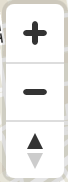
\includegraphics[width=0.3125in,height=\textheight,keepaspectratio]{./images/ultra-nav.png},

a \texttt{GeolocateControl}

\includegraphics[width=0.3125in,height=\textheight,keepaspectratio]{./images/ultra-loc.png}
and an \texttt{HTMLControl}.

To add these three controls, just copy and paste the following code
lines after the \texttt{options:} property and before the
\texttt{style:} in your query.

\phantomsection\label{annotated-cell-6}%
\begin{Shaded}
\begin{Highlighting}[]
\NormalTok{controls}\OperatorTok{:}\NormalTok{ \# }\OperatorTok{\textless{}}\DecValTok{1}\OperatorTok{\textgreater{}}
  \OperatorTok{{-}}\NormalTok{ type}\OperatorTok{:}\NormalTok{ NavigationControl \# }\OperatorTok{\textless{}}\DecValTok{2}\OperatorTok{\textgreater{}}
\NormalTok{    position}\OperatorTok{:}\NormalTok{ top}\OperatorTok{{-}}\NormalTok{right \# }\OperatorTok{\textless{}}\DecValTok{3}\OperatorTok{\textgreater{}}
  \OperatorTok{{-}}\NormalTok{ type}\OperatorTok{:}\NormalTok{ GeolocateControl \# }\OperatorTok{\textless{}}\DecValTok{4}\OperatorTok{\textgreater{}}
\NormalTok{    options}\OperatorTok{:}\NormalTok{ \# }\OperatorTok{\textless{}}\DecValTok{4}\OperatorTok{\textgreater{}}
\NormalTok{      positionOptions}\OperatorTok{:}\NormalTok{ \# }\OperatorTok{\textless{}}\DecValTok{4}\OperatorTok{\textgreater{}}
\NormalTok{        enableHighAccuracy}\OperatorTok{:} \KeywordTok{true}\NormalTok{ \# }\OperatorTok{\textless{}}\DecValTok{4}\OperatorTok{\textgreater{}}
\NormalTok{      trackUserLocation}\OperatorTok{:} \KeywordTok{true}\NormalTok{ \# }\OperatorTok{\textless{}}\DecValTok{5}\OperatorTok{\textgreater{}}
  \OperatorTok{{-}}\NormalTok{ type}\OperatorTok{:}\NormalTok{ HTMLControl \# }\OperatorTok{\textless{}}\DecValTok{6}\OperatorTok{\textgreater{}}
\NormalTok{    options}\OperatorTok{:}\NormalTok{ \# }\OperatorTok{\textless{}}\DecValTok{6}\OperatorTok{\textgreater{}}
\NormalTok{      html}\OperatorTok{:} \OperatorTok{\textgreater{}}\NormalTok{ \# }\OperatorTok{\textless{}}\DecValTok{7}\OperatorTok{\textgreater{}}
        \OperatorTok{\textless{}}\NormalTok{h1}\OperatorTok{\textgreater{}\textless{}}\NormalTok{center}\OperatorTok{\textgreater{}}\NormalTok{Green areas }\KeywordTok{in}\NormalTok{ Philadelphia}\OperatorTok{\textless{}/}\NormalTok{center}\OperatorTok{\textgreater{}\textless{}/}\NormalTok{h1}\OperatorTok{\textgreater{}}\NormalTok{ \# }\OperatorTok{\textless{}}\DecValTok{8}\OperatorTok{\textgreater{}}
\NormalTok{      css}\OperatorTok{:} \OperatorTok{\textgreater{}}\NormalTok{ \# }\OperatorTok{\textless{}}\DecValTok{9}\OperatorTok{\textgreater{}}
\NormalTok{        h1 \{ \# }\OperatorTok{\textless{}}\DecValTok{9}\OperatorTok{\textgreater{}}
          \DataTypeTok{position}\OperatorTok{:}\NormalTok{ fixed}\OperatorTok{;}\NormalTok{ \# }\OperatorTok{\textless{}}\DecValTok{9}\OperatorTok{\textgreater{}}
          \DataTypeTok{top}\OperatorTok{:} \DecValTok{0}\OperatorTok{;}\NormalTok{ \# }\OperatorTok{\textless{}}\DecValTok{9}\OperatorTok{\textgreater{}}
          \DataTypeTok{left}\OperatorTok{:} \DecValTok{0}\OperatorTok{;}\NormalTok{ \# }\OperatorTok{\textless{}}\DecValTok{9}\OperatorTok{\textgreater{}}
          \DataTypeTok{right}\OperatorTok{:} \DecValTok{0}\OperatorTok{;}\NormalTok{ \# }\OperatorTok{\textless{}}\DecValTok{9}\OperatorTok{\textgreater{}}
\NormalTok{        \} \# }\OperatorTok{\textless{}}\DecValTok{9}\OperatorTok{\textgreater{}}
\end{Highlighting}
\end{Shaded}

\begin{description}
\tightlist
\item[\circled{1}]
Adding the \texttt{controls:} property.
\item[\circled{2}]
Fist we add a type \texttt{NavigationControl}.
\item[\circled{3}]
Set the position of the control in the map window.
\item[\circled{4}]
Second we add a \texttt{GeolocateControl}.
\item[\circled{5}]
We enable the option to track the user location.
\item[\circled{6}]
Third we add the \texttt{HTMLControl} to include a title for the map.
\item[\circled{7}]
Open an html section.
\item[\circled{8}]
Include the text for the title betwen the
\texttt{\textless{}center\textgreater{}\ \textless{}/center\textgreater{}}.
\item[\circled{9}]
Style the title using css.
\end{description}

\begin{tcolorbox}[enhanced jigsaw, opacitybacktitle=0.6, colback=white, titlerule=0mm, colbacktitle=quarto-callout-note-color!10!white, coltitle=black, title=\textcolor{quarto-callout-note-color}{\faInfo}\hspace{0.5em}{Note}, leftrule=.75mm, breakable, bottomrule=.15mm, opacityback=0, bottomtitle=1mm, toprule=.15mm, toptitle=1mm, colframe=quarto-callout-note-color-frame, arc=.35mm, rightrule=.15mm, left=2mm]

These options will be visible only when you share the qyery as an
interactive map. See section 6 of this tutorial.

\end{tcolorbox}

\subsection{Customizing the popup
window}\label{customizing-the-popup-window}

Finally, another useful option to add is a customized popup window. This
window will appear when the viewer clicks or hover the mouse over one of
the elements from the query.

Here we add a customized popup window that shows the name and leisure
type and will appear when one hovers over the polygon.

Paste the code below under the \texttt{description:} property on your
query.

\phantomsection\label{annotated-cell-7}%
\begin{Shaded}
\begin{Highlighting}[]
\NormalTok{popupOnHover}\OperatorTok{:} \KeywordTok{true}\NormalTok{ \# }\OperatorTok{\textless{}}\DecValTok{1}\OperatorTok{\textgreater{}}
\NormalTok{popupTemplate}\OperatorTok{:} \StringTok{"\{\{tags.name\}\} {-} \{\{tags.leisure\}\}"}\NormalTok{ \# }\OperatorTok{\textless{}}\DecValTok{2}\OperatorTok{\textgreater{}}
\end{Highlighting}
\end{Shaded}

\begin{description}
\tightlist
\item[\circled{1}]
This activates the popup on hover. The defualt is when click.
\item[\circled{2}]
We only add the feature \texttt{name} and \texttt{leisure} type to the
popup.
\end{description}

\section{Complete query for an interactive
map}\label{complete-query-for-an-interactive-map}

You can copy and paste the code below on your query window. Remember to
zoom in to Philadelphia to have the correct bbox for the map configured
here. If you are working on a different area of interest, zoom in to
that area and change the \texttt{center:} and \texttt{zoom:} properties
on the YAML front-matter before running the query.

\begin{Shaded}
\begin{Highlighting}[numbers=left,,]
\OperatorTok{{-}{-}{-}}
\NormalTok{title}\OperatorTok{:}\NormalTok{ Recreational areas }\KeywordTok{in}\NormalTok{ Philadelphia}
\NormalTok{description}\OperatorTok{:}\NormalTok{ Map }\KeywordTok{of}\NormalTok{ all recreational areas }\KeywordTok{in}\NormalTok{ the city }\KeywordTok{of}\NormalTok{ Philadelphia}
\NormalTok{popupOnHover}\OperatorTok{:} \KeywordTok{true}
\NormalTok{popupTemplate}\OperatorTok{:} \StringTok{"\{\{tags.name\}\} {-} \{\{tags.leisure\}\}"}
\NormalTok{options}\OperatorTok{:}
\NormalTok{  center}\OperatorTok{:}\NormalTok{ [}\OperatorTok{{-}}\FloatTok{75.17474}\OperatorTok{,} \FloatTok{39.95880}\NormalTok{]}
\NormalTok{  zoom}\OperatorTok{:} \FloatTok{13.83}
\NormalTok{controls}\OperatorTok{:}
  \OperatorTok{{-}}\NormalTok{ type}\OperatorTok{:}\NormalTok{ NavigationControl}
\NormalTok{    position}\OperatorTok{:}\NormalTok{ top}\OperatorTok{{-}}\NormalTok{right}
  \OperatorTok{{-}}\NormalTok{ type}\OperatorTok{:}\NormalTok{ GeolocateControl}
\NormalTok{    options}\OperatorTok{:}
\NormalTok{      positionOptions}\OperatorTok{:}
\NormalTok{        enableHighAccuracy}\OperatorTok{:} \KeywordTok{true}
\NormalTok{      trackUserLocation}\OperatorTok{:} \KeywordTok{true}
  \OperatorTok{{-}}\NormalTok{ type}\OperatorTok{:}\NormalTok{ HTMLControl}
\NormalTok{    options}\OperatorTok{:}
\NormalTok{      html}\OperatorTok{:} \OperatorTok{\textgreater{}}
        \OperatorTok{\textless{}}\NormalTok{h1}\OperatorTok{\textgreater{}\textless{}}\NormalTok{center}\OperatorTok{\textgreater{}}\NormalTok{Green areas }\KeywordTok{in}\NormalTok{ Philadelphia}\OperatorTok{\textless{}/}\NormalTok{center}\OperatorTok{\textgreater{}\textless{}/}\NormalTok{h1}\OperatorTok{\textgreater{}}
\NormalTok{      css}\OperatorTok{:} \OperatorTok{\textgreater{}}
\NormalTok{        h1 \{}
          \DataTypeTok{position}\OperatorTok{:}\NormalTok{ fixed}\OperatorTok{;}
          \DataTypeTok{top}\OperatorTok{:} \DecValTok{0}\OperatorTok{;}
          \DataTypeTok{left}\OperatorTok{:} \DecValTok{0}\OperatorTok{;}
          \DataTypeTok{right}\OperatorTok{:} \DecValTok{0}\OperatorTok{;}
\NormalTok{        \}}
\NormalTok{style}\OperatorTok{:}
\NormalTok{  layers}\OperatorTok{:}                                          
    \OperatorTok{{-}}\NormalTok{ type}\OperatorTok{:}\NormalTok{ fill                                                  }
\NormalTok{      paint}\OperatorTok{:}                                          
\NormalTok{        fill}\OperatorTok{{-}}\NormalTok{color}\OperatorTok{:}
          \OperatorTok{{-}} \ControlFlowTok{case}
          \OperatorTok{{-}}\NormalTok{ [ }\OperatorTok{==,}\NormalTok{ [ }\KeywordTok{get}\OperatorTok{,}\NormalTok{ leisure ]}\OperatorTok{,} \StringTok{"park"}\NormalTok{ ]}
          \OperatorTok{{-}} \FunctionTok{rgb}\NormalTok{(}\DecValTok{159}\OperatorTok{,} \DecValTok{247}\OperatorTok{,} \DecValTok{7}\NormalTok{) \# green}
          \OperatorTok{{-}}\NormalTok{ [ }\OperatorTok{==,}\NormalTok{ [ }\KeywordTok{get}\OperatorTok{,}\NormalTok{ leisure ]}\OperatorTok{,} \StringTok{"playground"}\NormalTok{ ]}
          \OperatorTok{{-}} \FunctionTok{rgb}\NormalTok{(}\DecValTok{80}\OperatorTok{,} \DecValTok{163}\OperatorTok{,} \DecValTok{91}\NormalTok{) \# dark gren}
          \OperatorTok{{-}}\NormalTok{ [ }\OperatorTok{==,}\NormalTok{ [ }\KeywordTok{get}\OperatorTok{,}\NormalTok{ leisure ]}\OperatorTok{,} \StringTok{"garden"}\NormalTok{ ]}
          \OperatorTok{{-}} \FunctionTok{rgb}\NormalTok{(}\DecValTok{181}\OperatorTok{,} \DecValTok{159}\OperatorTok{,} \DecValTok{16}\NormalTok{) \# brown}
          \OperatorTok{{-}} \FunctionTok{rgb}\NormalTok{(}\DecValTok{0}\OperatorTok{,} \DecValTok{0}\OperatorTok{,} \DecValTok{0}\NormalTok{)}
  \KeywordTok{extends}\OperatorTok{:}\NormalTok{ https}\OperatorTok{:}\CommentTok{//styles.trailsta.sh/protomaps{-}light.json}
\OperatorTok{{-}{-}{-}}
\NormalTok{[bbox}\OperatorTok{:}\NormalTok{\{\{bbox\}\}]}\OperatorTok{;}
\NormalTok{(}
\NormalTok{  nwr[leisure}\OperatorTok{=}\NormalTok{park]}\OperatorTok{;}
\NormalTok{  nwr[leisure}\OperatorTok{=}\NormalTok{playground]}\OperatorTok{;}
\NormalTok{  nwr[leisure}\OperatorTok{=}\NormalTok{garden]}\OperatorTok{;}
\NormalTok{)}\OperatorTok{;}
\NormalTok{out geom}\OperatorTok{;}
\end{Highlighting}
\end{Shaded}

\begin{figure}[H]

{\centering \pandocbounded{\includegraphics[keepaspectratio]{./images/ultra-result1.png}}

}

\caption{Resulting Query Map}

\end{figure}%

\section{Sharing you Ultra map}\label{sharing-you-ultra-map}

The last step is to share your resulting map.

There are mutliple ways you can share it online, as a query or an
interactive map.

{01} \emph{Click on Share}

Click on the Share
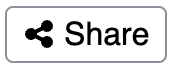
\includegraphics[width=\linewidth,height=0.3125in,keepaspectratio]{./images/ultra-share.png}

{02} \emph{Select how you want to share}

In the new window, select how you want to share the map.

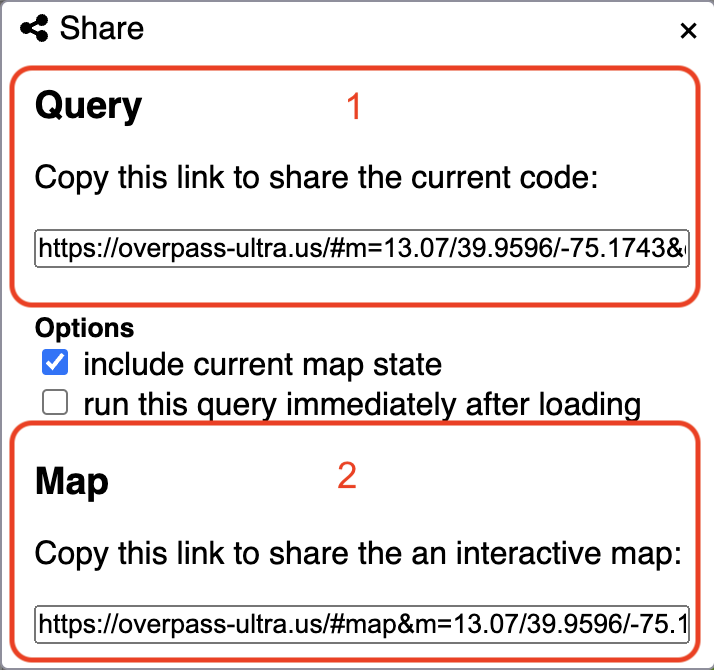
\includegraphics[width=3.125in,height=\textheight,keepaspectratio]{./images/ultra-share2.png}

\begin{enumerate}
\def\labelenumi{\arabic{enumi}.}
\tightlist
\item
  If you select to share as query, the link will open the map and query
  with all actions.
\end{enumerate}

\pandocbounded{\includegraphics[keepaspectratio]{./images/ultra-result1.png}}

\begin{enumerate}
\def\labelenumi{\arabic{enumi}.}
\setcounter{enumi}{1}
\tightlist
\item
  If you select to share as an interactive map, the link will open a
  mapview only, without the query window on the side.
\end{enumerate}

\pandocbounded{\includegraphics[keepaspectratio]{./images/ultra-result2.png}}

\section*{Attribution}\label{attribution}
\addcontentsline{toc}{section}{Attribution}

Open Geospatial Data by Felipe Valdez is licensed under CC BY-NC-SA 4.0




\end{document}
